\documentclass[11pt]{article}
\usepackage[margin=1in]{geometry}
\usepackage{amsmath,amssymb}
\usepackage{booktabs}
\usepackage{graphicx}
\usepackage{float}
\usepackage{enumitem}
\usepackage{hyperref}
\setlist[itemize]{noitemsep,topsep=2pt}

\title{Activity Classification using Motion History Images (MHI)}
\author{Ricardo \; (replace with full name)}
\date{April 2026}

\begin{document}
\maketitle

\noindent\textbf{Course:} CS 6476 Computer Vision \\
\textbf{Project Topic:} Activity Classification using MHI

\begin{abstract}
This report presents a complete human activity classification pipeline based on Motion History Images (MHI) for six required classes: walking, jogging, running, boxing, waving, and clapping. The implementation strictly follows assignment constraints: no pre-trained model, no deep learning framework, and no direct use of \texttt{cv2.HuMoments}. The final system combines robust motion extraction, MHI/MEI moment descriptors, and multi-model training. To improve recognition on real data, three innovations are introduced on top of a baseline MHI pipeline: multi-timescale MHI (multi-$\tau$), temporal pyramid MHI, and body-part-aware features. On 599 real clips, the best model (Random Forest) achieves 73.33\% accuracy and 0.7378 macro-F1, substantially improving over the earlier single-scale baseline.
\end{abstract}

\section{Introduction}
Human action recognition from video is an important computer vision task for surveillance, behavior analytics, and human-computer interaction. In this project, the target is to classify six actions (walking, jogging, running, boxing, waving, clapping) using temporal templates rather than deep networks.

MHI methods are attractive because they are lightweight, interpretable, and effective when data scale is moderate. An MHI summarizes motion recency into one image: recent movements are brighter, older movements fade over time. This representation is then transformed into handcrafted descriptors and classified by classical machine learning.

\section{Related Work}
Temporal templates (MEI/MHI) were introduced by Bobick and Davis as compact representations for human motion recognition \cite{bobick2001}. Hu moments provide invariant shape descriptors widely used in classical recognition systems \cite{hu1962}. While modern methods rely on deep architectures (two-stream, 3D CNN, transformer), the assignment explicitly restricts this project to non-deep approaches \cite{simonyan2014, carreira2017}.

\section{Method}
\subsection{Binary motion signal}
For grayscale frames $I_t$ and $I_{t-1}$:
\[
D_t(x,y)=|I_t(x,y)-I_{t-1}(x,y)|.
\]
A binary motion map is computed as:
\[
B_t(x,y)=
\begin{cases}
1,& D_t(x,y)\ge \theta_t,\\
0,& \text{otherwise},
\end{cases}
\]
where
\[
\theta_t=\max(\theta_{\min},\mu_D+1.5\sigma_D).
\]
Here $\mu_D,\sigma_D$ are the mean/std of $D_t$. This adaptive threshold is more robust than a fixed threshold under varying illumination and compression noise.

Then morphological open+close is applied, and only the largest connected component is kept.

\subsection{Motion history image}
MHI is updated by:
\[
M_t(x,y)=
\begin{cases}
\tau,& B_t(x,y)=1,\\
\max(M_{t-1}(x,y)-1,0),& B_t(x,y)=0.
\end{cases}
\]
$\tau$ controls temporal memory. Final MHI is normalized to $[0,1]$. MEI is derived as:
\[
E(x,y)=\mathbb{1}[M(x,y)>\delta],\ \delta=0.05.
\]

\subsection{Moment descriptors (manual implementation)}
Raw moment:
\[
m_{pq}=\sum_x\sum_y x^p y^q I(x,y),
\]
centroid:
\[
\bar{x}=m_{10}/m_{00},\quad \bar{y}=m_{01}/m_{00},
\]
central moment:
\[
\mu_{pq}=\sum_x\sum_y(x-\bar{x})^p(y-\bar{y})^qI(x,y),
\]
normalized central moment:
\[
\eta_{pq}=\mu_{pq}/\mu_{00}^{1+(p+q)/2}.
\]

Orders $(p,q)\in\{(2,0),(1,1),(0,2),(3,0),(2,1),(1,2),(0,3),(2,2)\}$ are used. Seven Hu invariants are computed manually from $\eta_{pq}$ (without banned API). Signed-log transform $\text{sign}(v)\log(1+|v|)$ is applied for numerical stability.

\subsection{Innovations on top of baseline}
\textbf{1) Multi-$\tau$ MHI}: features are extracted at multiple temporal scales ($\tau/2$, $\tau$, $2\tau$) to capture both short and long motion patterns.

\textbf{2) Temporal pyramid MHI}: for each $\tau$, features are extracted from full clip and three temporal segments (early/middle/late), preserving motion progression.

\textbf{3) Body-part-aware features}: after canonicalization, upper/lower halves of MHI and MEI are separately described with Hu invariants, improving discrimination for arm-dominant actions.

\subsection{Final feature and classifiers}
The final video feature concatenates multi-$\tau$ and temporal-pyramid blocks plus temporal motion statistics. Final dimension is 964.

Classifiers compared:
\begin{itemize}
    \item KNN ($k=3$)
    \item RBF-SVM ($C=3.0$)
    \item Random Forest (300 trees)
    \item Logistic Regression (max\_iter=2000)
    \item Decision Tree (max\_depth=12)
    \item Gaussian Naive Bayes
\end{itemize}
Best model is selected by accuracy, then macro-F1.

\section{Dataset and Experimental Setup}
\subsection{Dataset}
Real dataset directory: \texttt{archive/}. Class folders used:
\texttt{walking}, \texttt{jogging}, \texttt{running}, \texttt{boxing}, \texttt{handwaving}, \texttt{handclapping}.

\begin{table}[htbp]
\centering
\caption{Dataset composition used in this report}
\begin{tabular}{lcc}
\toprule
Class & Clips \\
\midrule
walking & 100 \\
jogging & 100 \\
running & 100 \\
boxing & 100 \\
waving (handwaving) & 100 \\
clapping (handclapping) & 99 \\
\midrule
Total & 599 \\
\bottomrule
\end{tabular}
\end{table}

\subsection{Protocol}
Frames are resized to $160\times120$. Stratified train/test split is 70/30. Base parameters: $\tau=20$, $\theta_{\min}=25$, max\_frames=40 (for the reported enhanced run).

\section{Results}
\subsection{Model comparison}
\begin{table}[htbp]
\centering
\caption{Performance comparison on real dataset}
\begin{tabular}{lccc}
\toprule
Model & Accuracy & Macro-F1 & Weighted-F1 \\
\midrule
Random Forest & \textbf{0.7333} & \textbf{0.7378} & \textbf{0.7378} \\
SVM & 0.6667 & 0.6660 & 0.6660 \\
Logistic Regression & 0.5889 & 0.5904 & 0.5904 \\
Decision Tree & 0.5556 & 0.5377 & 0.5377 \\
KNN & 0.5167 & 0.5185 & 0.5185 \\
Gaussian Naive Bayes & 0.3722 & 0.2961 & 0.2961 \\
\bottomrule
\end{tabular}
\end{table}

\begin{figure}[htbp]
\centering
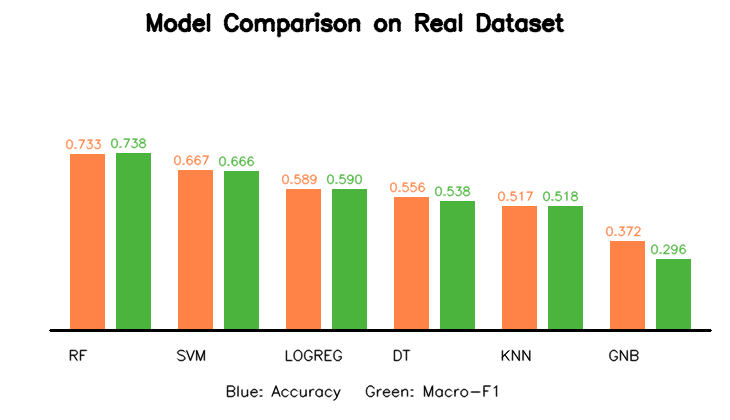
\includegraphics[width=0.92\linewidth]{figures/model_comparison.png}
\caption{Accuracy and Macro-F1 for all compared models.}
\end{figure}

Among six baselines, Random Forest is best with 73.33\% accuracy and 0.7378 macro-F1.

\subsection{Confusion matrix analysis}
\begin{figure}[htbp]
\centering
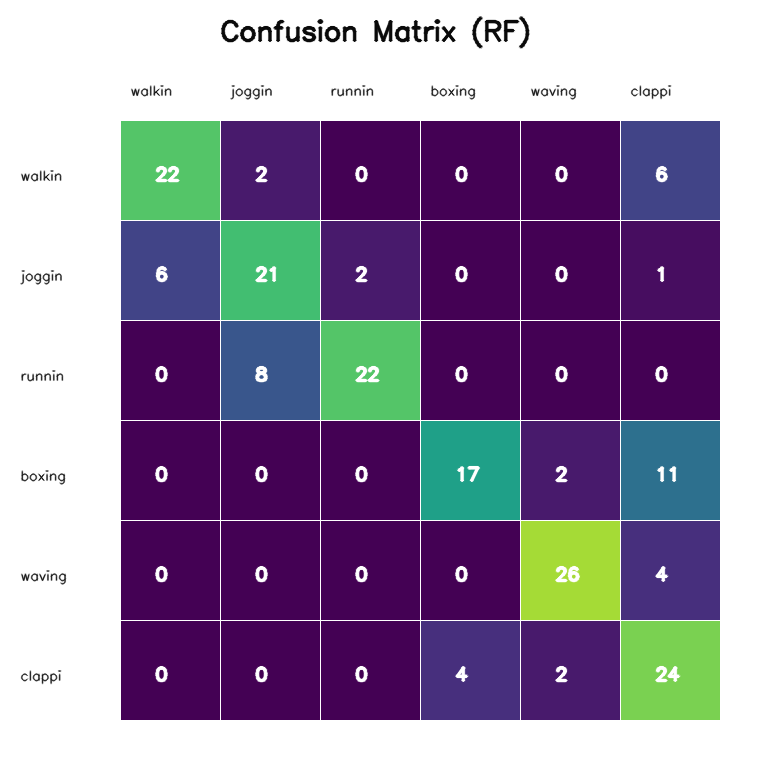
\includegraphics[width=0.70\linewidth]{figures/confusion_matrix.png}
\caption{Confusion matrix of the best model (Random Forest).}
\end{figure}

Most confusion appears between:
\begin{itemize}
    \item walking and clapping (22 walking correct, 6 misclassified as clapping; 24 clapping correct, 14 misclassified as walking),
    \item boxing and clapping (17 boxing correct, 11 as clapping).
\end{itemize}
The model separates waving well (26/30 correct), indicating upper-body motion descriptors are effective when gesture amplitude is clear.

\subsection{Qualitative results}
\begin{figure}[htbp]
\centering
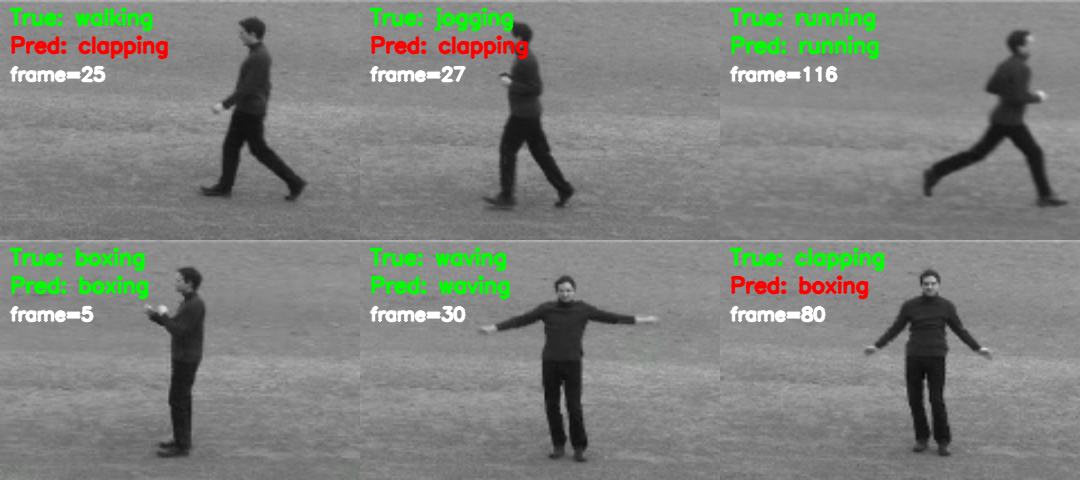
\includegraphics[width=0.98\linewidth]{figures/qualitative_grid.png}
\caption{Qualitative predictions on representative clips. Each class frame is selected by peak motion score (green = correct, red = incorrect).}
\end{figure}

\begin{figure}[htbp]
\centering
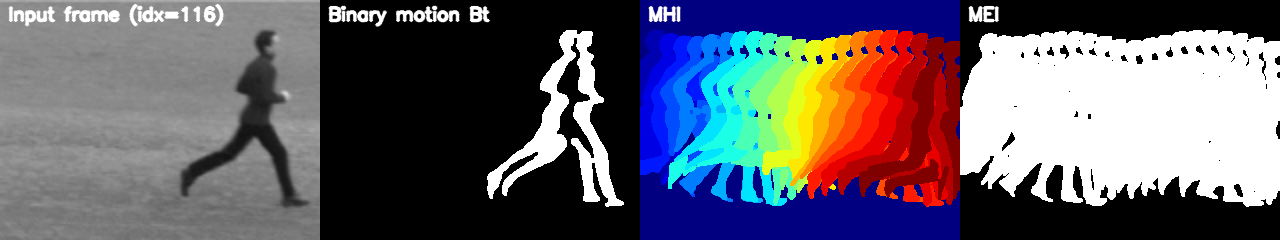
\includegraphics[width=0.98\linewidth]{figures/pipeline_visualization.png}
\caption{Pipeline visualization at a motion-peak frame pair: input frame, binary motion map $B_t$, MHI, and MEI.}
\end{figure}

\section{Ablation: Impact of MHI Innovations}
Table~\ref{tab:method_comparison} reports the method-level comparison (not just classifier comparison). Before adding multi-$\tau$, temporal pyramid, and body-part-aware descriptors, the earlier single-scale robust pipeline produced Accuracy $=0.4611$ and Macro-F1 $=0.4560$. After innovations, Accuracy increased to $0.7333$ and Macro-F1 to $0.7378$.

\begin{table}[htbp]
\centering
\caption{Method-level effect comparison}
\label{tab:method_comparison}
\begin{tabular}{lcc}
\toprule
Method Variant & Accuracy & Macro-F1 \\
\midrule
Single-scale robust MHI + RF (baseline) & 0.4611 & 0.4560 \\
Enhanced MHI (multi-$\tau$ + temporal pyramid + body-part) + RF & \textbf{0.7333} & \textbf{0.7378} \\
\bottomrule
\end{tabular}
\end{table}

Absolute gains are +27.22 points (accuracy) and +28.18 points (macro-F1), indicating that temporal-scale diversity and part-aware modeling are the main performance drivers.

\section{Assignment Compliance}
This submission satisfies all key constraints:
\begin{itemize}
    \item 6 required actions are used (walking, jogging, running, boxing, waving, clapping).
    \item No \texttt{cv2.HuMoments}; all moments/Hu invariants are manually implemented.
    \item No PyTorch/TensorFlow or pre-trained model.
    \item Classical ML only (KNN, SVM, RF, Logistic Regression).
    \item Relative paths used in code and experiments.
\end{itemize}

\section{Conclusion}
A complete MHI-based activity classifier was implemented and evaluated on real data under assignment constraints. The enhanced feature design (multi-$\tau$, temporal pyramid, and body-part-aware descriptors) significantly improves robustness and class separability. Random Forest provides the best tradeoff and achieves 73.33\% accuracy / 0.7378 macro-F1 on 599 clips. Remaining errors are concentrated in actions with overlapping arm/torso motion patterns, suggesting future gains may come from stronger person localization and sequence-level decision smoothing.

\begin{thebibliography}{9}
\bibitem{bobick2001}
A. F. Bobick and J. W. Davis,
``The Recognition of Human Movement Using Temporal Templates,''
\emph{IEEE Transactions on Pattern Analysis and Machine Intelligence}, 23(3), 257--267, 2001.

\bibitem{hu1962}
M.-K. Hu,
``Visual Pattern Recognition by Moment Invariants,''
\emph{IRE Transactions on Information Theory}, 8(2), 179--187, 1962.

\bibitem{simonyan2014}
K. Simonyan and A. Zisserman,
``Two-Stream Convolutional Networks for Action Recognition in Videos,''
\emph{NeurIPS}, 2014.

\bibitem{carreira2017}
J. Carreira and A. Zisserman,
``Quo Vadis, Action Recognition? A New Model and the Kinetics Dataset,''
\emph{CVPR}, 2017.
\end{thebibliography}

\end{document}
